\chapter{Entanglement, Density Matrices, and Locality}

This lecture opens in a deliberately corrective mood. Susskind had considered doing Bell's theorem immediately, but he backs off: Bell's theorem is lovely, but more important than the theorem itself is what it says. He wants first to get at what entanglement says about systems, and he even resists the temptation to call that ``the nature of reality.'' The first target is more precise. People say that entanglement means that two systems ``share a state.'' But a composite system always has a state. The real issue is whether the state of the whole is a product state.

That is why the lecture first turns to wave functions and then to density matrices. Once the state has been written in components, factorization becomes a meaningful statement; once one asks what Alice can know locally when the whole state is entangled, the density matrix becomes unavoidable. From there the lecture returns to the singlet, to measurement as entanglement, and finally to locality and Bell.

\section{Wave Functions As Coordinates In Hilbert Space}

The lecture begins by clearing away a possible confusion. A wave function may or may not have anything to do with literal waves. Historically the idea came from particles and wave motion, but logically it is much broader. A wave function is simply the coefficient of a state vector in a chosen basis.

Let us call the state of the system
\[
|\Psi\rangle.
\]
A basis is labeled by a complete set of commuting observables. We write those labels schematically as
\[
a,b,c,\ldots
\]
with the understanding that a single system may require one label or many. For a particle in ordinary space one may use the commuting coordinates $x,y,z$; for a single spin one convenient label is the value of $\sigma_z$; for two spins one needs two labels.

\begin{figure}[ht]
\centering

\includegraphics[width=0.72\textwidth]{lecture_07_figure_02.png}
\end{figure}

The board is partly obscured in this frame, but the structure is clear: first the abstract basis expansion, then the identification of the coefficient with the wave function. In standard form one writes
\begin{equation}
|\Psi\rangle
=
\sum_{a,b,c,\ldots}
\langle a,b,c,\ldots|\Psi\rangle\,
|a,b,c,\ldots\rangle.
\end{equation}
The coefficient is, by definition, the wave function. The board seems to write a capital $\Psi(a,b,c,\ldots)$ for this object; to keep the notation from fighting itself, we normalize the coefficient to lowercase and reserve $|\Psi\rangle$ for the state vector:
\begin{equation}
\psi(a,b,c,\ldots)=\langle a,b,c,\ldots|\Psi\rangle.
\end{equation}
Then the state may be rewritten as
\begin{equation}
|\Psi\rangle
=
\sum_{a,b,c,\ldots}
\psi(a,b,c,\ldots)\,
|a,b,c,\ldots\rangle.
\end{equation}

This is the whole point. The wave function is the set of expansion coefficients of the state vector in a basis, or equivalently the set of inner products of the state with the basis vectors. For a single spin in the $\sigma_z$ basis, $\psi$ is just the pair of amplitudes for up and down. For two spins, it is a function of two labels. The phrase ``wave function'' sounds special; the construction is not special at all.

A student remarks that this looks like a Fourier transform. Susskind answers carefully: changing basis is the analog of a Fourier transform. If we replace the $\sigma_z$ basis by the $\sigma_x$ basis, the state vector is the same but the coordinate description changes. In that sense the wave function is basis-dependent data attached to a basis-independent state.

\section{Expectation Values And Composite Systems}

At this point Susskind says he wants to introduce density matrices, and then immediately interrupts himself: first let us talk about expectation values. That pause matters. The algebra has to earn its keep before the later discussion of entanglement can become sharp.

Take an observable $L$. Its matrix elements in the basis $|a\rangle$ are
\begin{equation}
L_{a'a}=\langle a'|L|a\rangle.
\end{equation}
If
\[
|\Psi\rangle=\sum_a \psi(a)\,|a\rangle,
\qquad
\langle\Psi|=\sum_{a'} \psi^*(a')\,\langle a'|,
\]
then
\begin{align}
\langle L\rangle
&=\langle\Psi|L|\Psi\rangle \\
&=\left(\sum_{a'}\psi^*(a')\langle a'|\right)
L
\left(\sum_a \psi(a)|a\rangle\right) \\
&=\sum_{a',a}\psi^*(a')\,\langle a'|L|a\rangle\,\psi(a) \\
&=\sum_{a',a}\psi^*(a')\,L_{a'a}\,\psi(a).
\end{align}
This is one of the central formulas of the lecture. Expectation values reduce to wave functions, their complex conjugates, and matrix elements of observables.

Now let us enlarge the system. Suppose there are two subsystems, Alice's and Bob's. Let $a$ denote a complete set of labels for Alice and $b$ a complete set of labels for Bob. The basis of the combined system is then labeled by the pair $(a,b)$.

\begin{figure}[ht]
\centering

\includegraphics[width=0.56\textwidth]{lecture_07_figure_03.png}
\end{figure}

The board here is doing something pedagogical rather than algebraic: it is teaching the reader to climb from single-subsystem notation to composite notation. In clean form the same ladder is
\begin{align}
|a\rangle \\
|b\rangle \\
|a,b\rangle \\
|\Psi\rangle.
\end{align}
The point is that $(a,b)$ should be thought of as one compound label for one basis vector of the tensor-product space.

To keep close to the board, let us write the composite wave function as
\begin{equation}
\Psi(a,b)=\langle a,b|\Psi\rangle,
\end{equation}
so that
\begin{equation}
|\Psi\rangle=\sum_{a,b}\Psi(a,b)\,|a,b\rangle.
\end{equation}

Now suppose $L$ is an observable belonging to Alice and $M$ an observable belonging to Bob. In the composite space, Alice's observable acts on Alice's factor and leaves Bob's untouched:
\begin{equation}
L_{a'b';ab}=L_{a'a}\,\delta_{b'b}.
\end{equation}
Likewise Bob's observable acts trivially on Alice's factor:
\begin{equation}
M_{a'b';ab}=\delta_{a'a}\,M_{b'b}.
\end{equation}
This is the tensor-product structure in component form. Alice uses the same matrix she would have used if Bob did not exist, and the identity operator on Bob's Hilbert space records the fact that nothing happens on Bob's side.

From this, the expectation value of an Alice observable in a general composite state becomes
\begin{align}
\langle L_A\rangle
&=
\sum_{a',a,b',b}
\Psi^*(a',b')\,
L_{a'b';ab}\,
\Psi(a,b) \\
&=
\sum_{a',a,b}
\Psi^*(a',b)\,
L_{a'a}\,
\Psi(a,b).
\end{align}
This formula will later collapse into the reduced density matrix. But first it tells us how product states behave.

\section{Product States, Correlations, And The First Test For Entanglement}

A product state is now easy to define.

\begin{definition}
A composite state is a product state if its wave function factorizes:
\begin{equation}
\Psi(a,b)=\psi_A(a)\,\phi_B(b).
\end{equation}
\end{definition}

The lecture insists on the plainness of this. A product state is not mysterious. It simply means that Alice has a wave function of her own, Bob has a wave function of his own, and there is no additional joint structure.

Now let us prove the first useful fact. If the state is a product state, then Alice's local expectation values are exactly what they would have been if Bob were not present at all:
\begin{align}
\langle L_A\rangle
&=
\sum_{a',a,b}
\Psi^*(a',b)\,
L_{a'a}\,
\Psi(a,b) \\
&=
\sum_{a',a,b}
\psi_A^*(a')\,\phi_B^*(b)\,
L_{a'a}\,
\psi_A(a)\,\phi_B(b) \\
&=
\left(
\sum_{a',a}\psi_A^*(a')\,L_{a'a}\,\psi_A(a)
\right)
\left(
\sum_b \phi_B^*(b)\phi_B(b)
\right) \\
&=
\sum_{a',a}\psi_A^*(a')\,L_{a'a}\,\psi_A(a),
\end{align}
since Bob's wave function is normalized:
\[
\sum_b \phi_B^*(b)\phi_B(b)=1.
\]
Thus Bob drops out completely. In a product state Alice's statistics are Alice's statistics.

The same argument gives Bob's formula:
\begin{equation}
\langle M_B\rangle
=
\sum_{b',b}\phi_B^*(b')\,M_{b'b}\,\phi_B(b).
\end{equation}
So product states really are what they sound like: as far as local measurements are concerned, neither party knows anything about the other.

The next step is to look at the product of an Alice observable and a Bob observable. For a product state,
\begin{align}
\langle L_A M_B\rangle
&=
\sum_{a',a,b',b}
\psi_A^*(a')\,\phi_B^*(b')\,
L_{a'a}M_{b'b}\,
\psi_A(a)\,\phi_B(b) \\
&=
\left(
\sum_{a',a}\psi_A^*(a')\,L_{a'a}\,\psi_A(a)
\right)
\left(
\sum_{b',b}\phi_B^*(b')\,M_{b'b}\,\phi_B(b)
\right) \\
&=
\langle L_A\rangle\,\langle M_B\rangle.
\end{align}

This is the quantum version of an entirely familiar classical statement: the average of a product equals the product of averages only when the variables are independent. That suggests the first operational test for entanglement. Define the correlation
\begin{equation}
C(L,M)=\langle LM\rangle-\langle L\rangle\langle M\rangle.
\end{equation}
Within the pure-state discussion of this lecture, if one can find an Alice observable $L$ and a Bob observable $M$ such that $C(L,M)\neq 0$, then the state is not a product state. That is the first clear sign of entanglement.

\subsection{Question \& Answer}

What does $LM$ mean here? It does not mean ``measure $M$ and then measure $L$.'' This is one of the local obstacles in the room, and Susskind pauses to remove it. $LM$ is the product of operators. It means: first let $M$ act on the vector, then let $L$ act on the result. That is a mathematical operation in the space of states, not the physical act of measurement.

In the present setup, $L$ belongs to Alice and $M$ belongs to Bob, so they act on different tensor factors and therefore commute:
\begin{equation}
[L,M]=0.
\end{equation}
That is true whether or not the state is entangled. The order of the operator product does not matter, but that still does not turn $LM$ into a time-ordered sequence of measurements. Detectors and apparatuses measure. Operators act on vectors.

\section{The Singlet State And Knowing The Whole But Not The Parts}

The abstract correlation criterion now needs a state with some bite. The lecture returns to the singlet:
\begin{equation}
|\Psi_{\mathrm{sing}}\rangle
=
\frac{1}{\sqrt2}
\left(
|\uparrow\downarrow\rangle
-
|\downarrow\uparrow\rangle
\right).
\end{equation}
We keep the lecture's slot order: Bob first, Alice second. This is not a product state.

In the $z$ basis, the local expectation values are obvious. Bob is up half the time and down half the time, and so is Alice:
\begin{equation}
\langle \sigma_z\rangle=0,
\qquad
\langle \tau_z\rangle=0.
\end{equation}
But the product is definite:
\begin{equation}
\langle \sigma_z\tau_z\rangle=-1.
\end{equation}
Each term in the singlet has opposite spins, so the product is always $-1$.

The lecture then recalls the less obvious but equally important fact that the same thing is true in the $x$ and $y$ directions. One finds
\begin{equation}
\langle \sigma_i\rangle=\langle \tau_i\rangle=0,
\qquad
\langle \sigma_i\tau_i\rangle=-1,
\qquad
i=x,y,z.
\end{equation}
Thus each spin by itself is maximally uncertain, while the joint products are perfectly fixed.

This is the real punchline. For an ordinary pure state of a single spin, there is always some axis along which the spin is definite. The singlet destroys that possibility locally. No matter what direction Bob measures, his average spin is zero; the same is true for Alice. And yet the combined system is as definite as quantum mechanics allows it to be. We know the whole and know nothing definite about the parts. That is the oddity of entanglement in its sharpest form.

The lecture reformulates the same fact with the operator
\begin{equation}
\sigma\!\cdot\!\tau
=
\sigma_x\tau_x+\sigma_y\tau_y+\sigma_z\tau_z.
\end{equation}
The singlet is an eigenvector of each separate product with eigenvalue $-1$:
\begin{equation}
\sigma_x\tau_x\,|\Psi_{\mathrm{sing}}\rangle
=
\sigma_y\tau_y\,|\Psi_{\mathrm{sing}}\rangle
=
\sigma_z\tau_z\,|\Psi_{\mathrm{sing}}\rangle
=
-|\Psi_{\mathrm{sing}}\rangle,
\end{equation}
and therefore
\begin{equation}
(\sigma\!\cdot\!\tau)\,|\Psi_{\mathrm{sing}}\rangle
=
-3\,|\Psi_{\mathrm{sing}}\rangle.
\end{equation}

There is an instructive subtlety here. The operator $\sigma\!\cdot\!\tau$ is a perfectly good Hermitian operator, but it cannot be measured merely by having Alice measure $\tau_x,\tau_y,\tau_z$ and Bob measure $\sigma_x,\sigma_y,\sigma_z$ separately, because Alice cannot simultaneously measure $\tau_x,\tau_y,\tau_z$. So this operator exists cleanly in Hilbert space, but measuring it requires a genuinely different joint apparatus.

The lecture then answers the natural laboratory question: how would one prepare the singlet? The answer is by energy. When two spins are brought together, $\sigma\!\cdot\!\tau$ appears as part of the Hamiltonian. The singlet is the lower-energy state; the three triplet states lie above it. If the system can lose energy by emitting a photon, a phonon, or by any other relaxation mechanism, it tends toward the singlet. One may therefore prepare the state by bringing the spins together, waiting until the higher components have decayed away, and then separating the spins again without twisting them. This is not a side story. It is the physical route by which the abstract singlet becomes an actual state in the laboratory.

\section{Density Matrices As Alice's Complete Local Description}

At this stage the lecture reaches the limit of wave functions as local descriptions. If the whole state is entangled, Alice cannot in general peel off a wave function for her subsystem alone. What, then, can she know? The answer is: not a local wave function, but a local density matrix.

\begin{figure}[ht]
\centering

\includegraphics[width=0.68\textwidth]{lecture_07_figure_04.png}
\end{figure}

The transcript is garbled just before this point, but once the definition appears the argument is perfectly clear. Start from the general expectation value of an Alice observable:
\begin{align}
\langle L_A\rangle
&=
\sum_{a',a,b}
\Psi^*(a',b)\,
L_{a'a}\,
\Psi(a,b) \\
&=
\sum_{a',a}
\left[
\sum_b \Psi^*(a',b)\Psi(a,b)
\right]
L_{a'a}.
\end{align}
The bracketed quantity depends only on Alice's labels. That is the reduced density matrix:
\begin{equation}
\rho_A(a',a)=\sum_b \Psi^*(a',b)\,\Psi(a,b).
\end{equation}
With that definition,
\begin{equation}
\langle L_A\rangle
=
\sum_{a',a}\rho_A(a',a)\,L_{a'a}.
\end{equation}
The spoken lecture remarks that one of the indices may have been written backward on the board. That is not the essential point. The essential point is that once $\rho_A$ is known, Alice can forget Bob completely for the purpose of predicting all of her local measurement statistics.

If the total state happens to be a product state,
\[
\Psi(a,b)=\psi_A(a)\phi_B(b),
\]
then the reduced density matrix simplifies immediately:
\begin{align}
\rho_A(a',a)
&=
\sum_b \psi_A^*(a')\phi_B^*(b)\,\psi_A(a)\phi_B(b) \\
&=
\psi_A^*(a')\psi_A(a)\sum_b |\phi_B(b)|^2 \\
&=
\psi_A^*(a')\psi_A(a).
\end{align}
So for a product state the density matrix is built entirely out of Alice's own wave function.

To make the matrix action transparent, it is convenient to regard the same object in ordinary row-column form. Then the entries are
\begin{equation}
\rho_{aa'}=\psi_A(a)\psi_A^*(a'),
\end{equation}
and the matrix-times-column-vector step visible on the board becomes
\begin{equation}
\sum_{a'}\rho_{aa'}\,\psi_A(a')=\psi_A(a).
\end{equation}

\begin{proposition}
If the composite state is a product pure state, then Alice's reduced density matrix has one and only one nonzero eigenvalue, equal to $1$. Every vector orthogonal to Alice's wave function is an eigenvector with eigenvalue $0$.
\end{proposition}

\begin{proof}
For a product state,
\[
\rho_{aa'}=\psi_A(a)\psi_A^*(a').
\]
Act on the column vector $\psi_A(a')$:
\begin{align}
\sum_{a'}\rho_{aa'}\,\psi_A(a')
&=
\sum_{a'}\psi_A(a)\psi_A^*(a')\psi_A(a') \\
&=
\psi_A(a)\sum_{a'}|\psi_A(a')|^2 \\
&=
\psi_A(a),
\end{align}
using normalization. Thus $|\psi_A\rangle$ is an eigenvector with eigenvalue $1$.

Now take any vector $|\widetilde\psi\rangle$ orthogonal to $|\psi_A\rangle$. Then
\[
\sum_{a'}\psi_A^*(a')\widetilde\psi(a')=0,
\]
and therefore
\begin{align}
\sum_{a'}\rho_{aa'}\,\widetilde\psi(a')
&=
\sum_{a'}\psi_A(a)\psi_A^*(a')\widetilde\psi(a') \\
&=
\psi_A(a)\sum_{a'}\psi_A^*(a')\widetilde\psi(a') \\
&=
0.
\end{align}
So every vector orthogonal to $|\psi_A\rangle$ has eigenvalue $0$. There is one eigenvalue $1$ and all the rest vanish.
\end{proof}

This gives the lecture's practical criterion. A product pure state has exactly one nonzero eigenvalue. An entangled state has more than one nonzero eigenvalue. The maximally entangled case is the one in which the nonzero eigenvalues are all equal; if Alice's Hilbert space has dimension $n$, that means
\begin{equation}
\lambda_i=\frac{1}{n}.
\end{equation}
For the singlet,
\begin{equation}
\rho_A
=
\frac12
\begin{pmatrix}
1 & 0 \\
0 & 1
\end{pmatrix},
\end{equation}
so
\begin{equation}
\operatorname{spec}(\rho_A)=\left\{\frac12,\frac12\right\}.
\end{equation}
That is maximal entanglement for a two-dimensional subsystem.

The lecture states the criterion in a deliberately rough way: one nonzero eigenvalue means no entanglement, several nonzero eigenvalues mean entanglement, and equal eigenvalues mean maximal entanglement. That is the operational content. One should not overread the casual remark that ``in general'' all eigenvalues are nonzero; the real test is that more than one nonzero eigenvalue has appeared.

\section{Measurement As Entanglement, Then Locality And Bell}

Having finished the density-matrix calculation, Susskind says, in effect, let us do it again. This time the composite system will not be Alice and Bob, but a system and an apparatus. The point is to show that measurement is not something added on top of entanglement. Measurement is an entangling process.

Take a detector with two states, $|0\rangle$ and $|1\rangle$. The detector begins in a known neutral state, $|0\rangle$; otherwise it is not ready to measure anything. Let the system be a spin with states $|u\rangle$ and $|d\rangle$. The interaction is idealized by the rule
\begin{equation}
|u,0\rangle\to|u,1\rangle,
\qquad
|d,0\rangle\to|d,0\rangle.
\end{equation}
The up spin activates the detector, the down spin does not.

Now feed in a superposed spin:
\begin{equation}
(\alpha|u\rangle+\beta|d\rangle)\otimes|0\rangle
\to
\alpha|u,1\rangle+\beta|d,0\rangle.
\end{equation}
The final state is not a product state. It is entangled. By looking at the apparatus one can tell what the spin did. That is exactly what a measurement is supposed to accomplish.

From one point of view, this is familiar laboratory language: the apparatus stores a record. From another point of view, it is just the unitary quantum mechanics of a larger system. If we talk only about the spin, we say the wave function has collapsed to the branch recorded by the apparatus. If we include the apparatus in the system, then no collapse has yet occurred; there is only the growth of entanglement.

The lecture then keeps enlarging the system. After apparatus comes eye, then brain, then Wigner looking at Schr\"odinger. The world becomes an onion: system inside apparatus inside observer inside a larger observer. Wherever one chooses to stop enlarging the system, one may speak of collapse outside that line; inside the line, the description is again ordinary quantum mechanics and entanglement. Susskind does not try to settle the interpretation. His point is more disciplined: wherever one draws the line, the predictions remain consistent.

This is also where weak measurement enters naturally. If the coupling between system and apparatus is too weak, the entanglement is only partial and the apparatus stores only partial information. Or the apparatus may record the information well while the later chain from eye to brain is noisy. Those are different failures. In one case the entangling interaction itself is weak; in the other case the record exists but is not cleanly transmitted onward.

Now the lecture turns to locality. Einstein's complaint was not foolishness; it was that quantum mechanics allows one to know everything about a composite system and yet nothing definite about its parts. But the phrase ``spooky action at a distance'' easily misleads. In ordinary physics, action at a distance means something concrete: the ability to affect distant outcomes immediately, in other words the ability to send a signal.

Entanglement does not do that. If Alice and Bob separate to distant locations and Bob performs any local experiment on his subsystem, Alice's local statistics do not suddenly change. In density-matrix language, the claim is that Bob-only interventions leave Alice's unconditioned local state unchanged:
\begin{equation}
\rho_A'=\rho_A.
\end{equation}
This equation is schematic rather than fully derived here, but it captures the lecture's claim: until classical information reaches Alice, Bob's local action does not alter the probabilities Alice assigns to her own outcomes.

The lecture makes this concrete by imagining many entangled pairs. Bob may measure $\sigma_z$ on one pair, $\sigma_x$ on a second, and $\sigma_y$ on a third. Unless he communicates the results, Alice's own ensemble remains statistically unchanged.

\begin{figure}[ht]
\centering

\includegraphics[width=0.78\textwidth]{lecture_07_figure_06.png}
\end{figure}

The board sketch is documentary rather than polished, and it is worth keeping for exactly that reason. A modest redraw clarifies the stable structure without pretending to replace the original evidence:

\begin{figure}[ht]
\centering
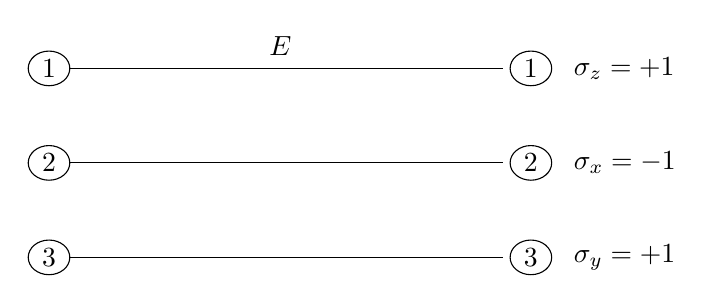
\begin{tikzpicture}[x=1.2cm,y=1cm]
\draw (0,0) circle (0.22) node {1};
\draw (0,-1.2) circle (0.22) node {2};
\draw (0,-2.4) circle (0.22) node {3};

\draw (0.22,0) -- (4.8,0);
\draw (0.22,-1.2) -- (4.8,-1.2);
\draw (0.22,-2.4) -- (4.8,-2.4);

\node at (2.45,0.28) {$E$};

\draw (5.1,0) circle (0.22) node {1};
\draw (5.1,-1.2) circle (0.22) node {2};
\draw (5.1,-2.4) circle (0.22) node {3};

\node[anchor=west] at (5.45,0) {$\sigma_z=+1$};
\node[anchor=west] at (5.45,-1.2) {$\sigma_x=-1$};
\node[anchor=west] at (5.45,-2.4) {$\sigma_y=+1$};
\end{tikzpicture}
\end{figure}

The lower label $\sigma_y=+1$ is supported by the aligned subtitle window rather than by a fully legible handwritten board line. That is enough to complete the logic of the example. Bob's different axis choices do nothing to Alice's statistics until the ordinary message arrives. Once it does arrive, Alice may choose to measure along the same axes and she will find the opposite answers, pair by pair.

\subsection{Question \& Answer}

If Bob measures first, when does Alice's density matrix actually change?

As far as Alice is concerned, it changes when Alice receives information that Bob obtained a result. Before that, her density matrix encodes only the probabilities locally available to her, and those probabilities have not changed. After the telegram arrives, she updates her state assignment. That update can be described in the language of collapse if one likes, but it is not an instantaneous physical influence reaching across space. It occurs only after enough time has passed for the message to get there.

That settles no-signaling, but it does not settle Bell. What, then, is Bell's issue? The lecture answers with a game about classical computers.

A single classical computer can simulate a single spin. It stores the amplitudes
\begin{equation}
|\psi\rangle=\alpha_u|u\rangle+\alpha_d|d\rangle,
\qquad
|\alpha_u|^2+|\alpha_d|^2=1,
\end{equation}
updates them by solving the Schr\"odinger equation, converts them into probabilities when the measure button is pressed, uses a random number generator to produce an outcome, and then updates the stored state so that it agrees with the outcome just recorded. For one spin, this is a perfectly good classical simulation. The difference between classical and quantum mechanics is not randomness by itself.

If the two-spin state is a product state, then two separated classical computers can simulate it as well: one keeps track of Alice, the other of Bob, and the two do not need to talk to each other. But if the state is entangled, Bell's point is that this no longer works. One may bring the computers together to prepare correlated data, but after separation that is still not enough. Synchronizing the random number generators in advance is not enough. To reproduce entangled quantum statistics, the separated classical machines would have to keep communicating. Hidden wires would have to continue to connect them.

That, in Susskind's language, is what Bell's theorem really says. An entangled quantum system cannot be simulated by genuinely separated classical bookkeeping. A single classical computer can do the job because all its parts can talk to all other parts. Two separated classical computers cannot, unless one secretly lets them continue exchanging information. The nonclassicality lies there.

And yet even that is not the same as faster-than-light signaling by Alice and Bob themselves. If one restricts oneself to the operations that quantum mechanics actually allows, one still cannot exploit the entangled setup to send arbitrary messages instantaneously. Bell does not restore ordinary action at a distance in the old sense. It says instead that the classical separated simulation picture is too small.

The lecture closes with an ensemble-level diagnostic that fits the entire chapter. Bob by himself cannot diagnose entanglement from one pair. But if he is given many identically prepared copies, he can search over directions in space. For a product state, some axis will eventually reveal a definite local polarization: measure enough copies along that axis and the same answer keeps returning. For an entangled state like the singlet, no such axis exists. Every direction remains locally random. That is the local face of the statement that Bob does not possess a pure local wave function, only a reduced density matrix.

\section{Summary}

The lecture unfolds in a very specific order. First, entanglement is not the vague statement that two systems ``share a state.'' A composite system always has a state; the real issue is whether it is a product state. Second, wave functions make that question explicit by turning states into coefficients in a basis. Third, product states force local expectation values to decouple, and the failure of that decoupling is the first operational sign of entanglement. Fourth, the singlet shows the extreme case: each part is maximally indefinite, while the whole has sharp joint structure.

Fifth, the reduced density matrix is the right local object when the whole state is entangled. For a product pure state it has one nonzero eigenvalue, equal to $1$; for the singlet it has two equal eigenvalues, $\frac12$ and $\frac12$. Sixth, measurement itself is an entangling interaction between system and apparatus, and one may push that logic outward through apparatus, eye, brain, and observer without finding a sharp boundary. Finally, locality survives in the operational sense that Bob cannot change Alice's statistics faster than light, but Bell still tells us that entangled systems refuse to be reproduced by genuinely separated classical simulations. The oddity remains exactly where Susskind wants it: quantum mechanics can allow full knowledge of a whole while withholding any definite local story about the parts.